\section{Video Compression}
Video compression can offer a significant reduction in the amount of data that needs to be stored or transmitted.
Beyond the methods used by image compression, video compression can exploit the temporal redundancy between frames.
That is, the fact that the content of two consecutive frames is often very similar.

In video compression, the frames are divided into three categories: Intra (I), Prediction (P) and Bi-Directional (B) frames \cite{vijayanagarBframesDifferencesUse2020}.
Intra frames are encoded using only the information in the frame itself in a similar manner to image compression \cite{vijayanagarBframesDifferencesUse2020}.
Prediction frames are encoded using the information in one or more previous frames as shown in Figure \ref{fig:multiple_reference_frames}.
Bi-Directional frames are encoded using both the previous and the future frames as illustrated in Figure \ref{fig:ipb_frames} \cite{vijayanagarBframesDifferencesUse2020}.
For P and B frames motion vectors are used to describe the movement of objects in the frame \cite{vijayanagarBframesDifferencesUse2020}.

As video encoding and decoding is computationally intensive, systems often use dedicated hardware to perform the encoding and decoding.
The \gls{h265} encoder used in this project is implemented in hardware on the \jx \cite[16]{nvidiaNVIDIAJetsonAGX2019}.

\begin{figure}
    \centering
    
\includegraphics[width=\textwidth]{figures/encoding/multiple_references.pdf}
    \caption{Visualization of the use of multiple reference Frames.}
    \label{fig:multiple_reference_frames}
\end{figure}

\begin{figure}
    \centering
    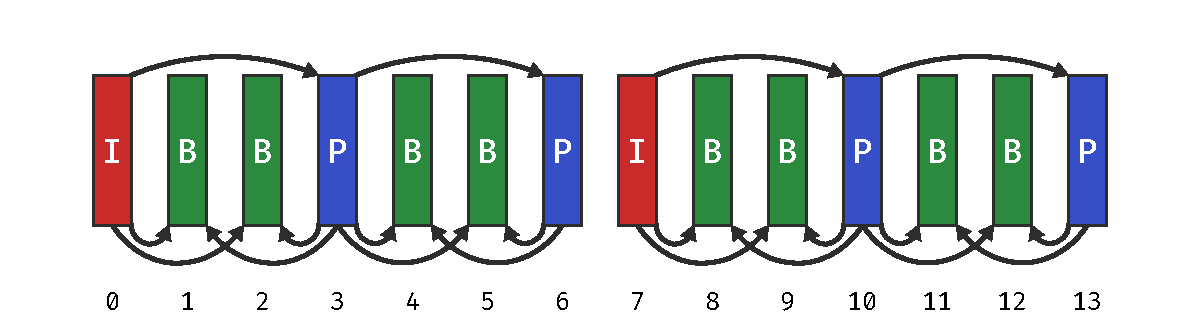
\includegraphics[width=\textwidth]{figures/encoding/ipb_frames.pdf}
    \caption{Visualization of Intra (I), Prediction (P) and Bi-Directional (B) frames.}
    \label{fig:ipb_frames}
\end{figure}

